\documentclass[12pt]{article}
\usepackage{ulem}
\usepackage{apacite}
\usepackage{amsmath}
\usepackage{amssymb}
\usepackage{graphicx}
\usepackage{enumerate}
\usepackage{algorithm}
\usepackage{algorithmicx}
\usepackage{algpseudocode}
\usepackage{setspace}
\usepackage[rgb]{xcolor}
\usepackage[numbers]{natbib}
\usepackage[a4paper,margin=2cm]{geometry}
\usepackage[colorlinks=true, urlcolor=blue, linkcolor=blue, citecolor=blue]{hyperref}

\newtheorem{lemma}{Lemma}[section]
\newtheorem{theorem}{Theorem}[section]
\newtheorem{corollary}{Corollary}[section]
\newtheorem{definition}{Definition}[section]

\begin{document}
\begin{spacing}{1.15}
\title{\bf Final Project Report: The Hanabi Game}
\author{Xiuhan Wang, Jing Wei}
\date{\today}
\maketitle

\section{Introduction}
The Hanabi game is a benchmark challenge in fully cooperative games of imperfect information. It's very different from adversarial two-player zero-sum games which have been studied more. But non-zero-sum scenarios are more important in real life.

In this game of limited communication, players convey information by choosing actions from a few options. Therefore to understand others' messages, the player must reason about beliefs and intentions of other players. Such theory of mind reasoning is crucial in more general collaborative efforts, especially those with human partners.\cite{bard2020the}

\section{Rules of the Hanabi Game}

\textsl{Hanabi} is a game for two to five players. Each player holds four cards in his hand (or five if less than four players). Everyone can see all others' cards but not that of himself. Each card has a rank (1--5) and a color (red, green, blue, yellow or white). There are three 1s, two 2s, 3s, 4s and a 5 of each color; hence 50 cards in total. The players are fully cooperative---they want to play cards to build five stacks, one for each color, going consecutively from 1. The goal is to maximize the score, which is the total number of cards in the stack.

Players take turns to play. In one's turn, he must take exactly one of the following actions:

\begin{itemize}
\item \textbf{Hint.} To give a hint to others, the player chooses a color or a rank, then point out all cards matching that color or rank in another player's hand. Only ranks and colors that are present in the other player's hand can be chosen. To limit the number of hints, the group has initially eight information tokens and a token is consumed when giving a hint.
\item \textbf{Discard.} When there are less than eight information tokens, he can discard a card from his hand, draw a new card from the deck and recover an information token. The discarded card is visible to all players and the newly drawn card is visible only to all other players.
\item \textbf{Play.} The player can choose a card from his hand and try to put it in the stacks. It's successful if the rank is exactly one larger than the top of the stack corresponding to the color. If it's successful, put the card on the top of that stack. Recover one information token if there are less than eight and the rank played is 5. If the play is unsuccessful, discard the card and the group loses one life. When three lives are lost, the game ends immediately. Whether successful or not, the player draws a new card from the deck.
\end{itemize}

\begin{figure}[H]
\centerline{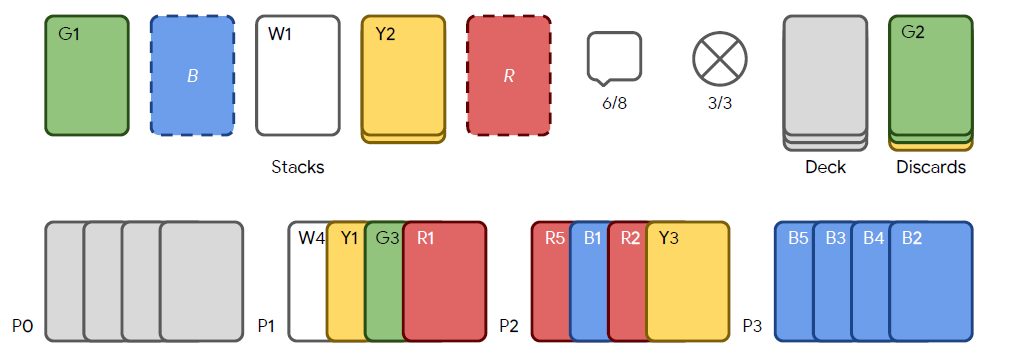
\includegraphics[width=6in]{fig1.png}}
\caption{An example of a four player Hanabi game from the point of view of player 0 (cite from \cite{bard2020the}).}
\label{Fig1}
\end{figure}

\section{Previous Methods on Hanabi}

The Hanabi game was proved \textsf{NP}-hard even if all hidden information is revealed.\cite{baffier2017hanabi} The hand-coded mathematical ``hat guessing game'' strategy\cite{cox2015how} held state-of-the-art results from March 2016 until December 2019. In five-player games, it almost achieved the best performance resulted by a cheating strategy where each player sees his own cards and uses the information strategy. However, it performed badly in the two-player setting\cite{bouzy2017playing}; and it is not generalizable to similar games. A Monte-Carlo tree search algorithm is given by \cite{walton-rivers2017evaluating}; but the performance is still not very good.

Foerster and Song proposed a method of Bayesian action decoder (BAD)\cite{foerster2018bayesian}. The key idea is a joint public belief over players' private features to resolve recursive belief over beliefs, and sampling a deterministic partial policy to resolve the dilemma between informative actions and stochastic actions for exploration. BAD worked well in the two-player setting. Hu and Foerster continued to optimize BAD to SAD\cite{hu2020simplified} and incorperated search into SPARTA\cite{lerer2020improving} to achieve a new state-of-the-art result.

Then they come up with the method called ``other-play'' (OP) that work well on the zero-shot coordination scenario of the game. Previous studies on MARL usually focus on the self-play (SP) setting where agents are trained and tested both against with themselves, but agents naively trained by SP could do arbitrarily bad when paired with a partner they’re not trained with. OP trains the agent with a copy of itself that is randomly permuted according to the symmetries in the game; hence it reduces the tendency towards arbitrary symmetry breaking. Agents trained with OP perform well when tested by cross-play, and also cooperate well with human.

Our work aims to be a better substitute for OP. Intuitively, the optimal strategies for symmetric games should be the same. As an analog, the convolutional neural network uses a symmetric network for training. We apply this idea to the network and reduce the network size by the symmetry group size.

\section{Zero-Shot Coordination}

Zero-shot coordination is the scenario where players are paired with strangers they're not trained with, and must quickly coordinate to cooperate. Consider the following \textsl{lever coordination game}: two players, who don't know each other, will choose two levers independently. If they choose the same, they can get the reward of that lever. Otherwise, the reward is 0. In Figure \ref{Fig2} (a), obviously the only strategy is to pick a lever at random, with expected reward 0.1. However in (b), if they both pick a 1-lever, the expected reward is 0.11. But if they both pick the 0.9-lever, they get higher reward 0.9.

\begin{figure}[H]
\centerline{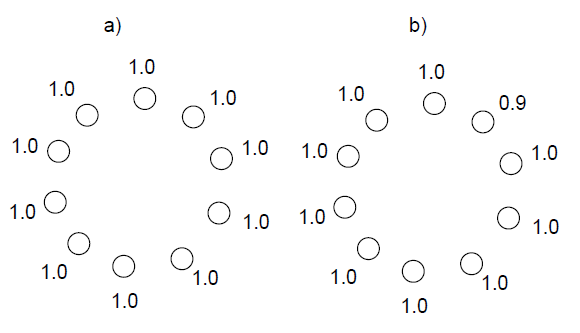
\includegraphics[width=4in]{fig2.png}}
\caption{An example of a lever coordination game (cite from \cite{hu2020other}).}
\label{Fig2}
\end{figure}

Agents trained by self-play would quickly reach a convention to pick the same lever. This gives the highest payoff 1 and is fine when playing with the same partner they're trained with. We see, in self-play, agents often use coordinated symmetry breaking to get higher payoffs, but this doesn't work and will be disastrous in the zero-shot coordination setting.

Similarly in Hanabi, the 5 colors are symmetric and thus indistinguishable. Self-play bots' strategies often involves conventions like ``hinting yellow means discarding the first card``. This would coordinate badly with another agent whose convention is ``hinting blue means discarding the first card'', which has the same chance of being adopted by self-play as the strategy.

\section{Other Play}
\renewcommand\S{{\mathcal S}}
\renewcommand\O{{\mathcal O}}
\newcommand\A{{\mathcal A}}

Arbitrary symmetries breaking is harmful in zero-shot coordination. Foerster et al.' proposed a method called \textsl{other-play} (OP)\cite{hu2020other} to alleviate this problem.

The symmetries in the MDP can be described as a isomorphism over states $\S$, observations $\A$ and actions $\O$ that keeps the transition function $P$, the reward $R$ and the observation function $O$ invariant.
\begin{align*}
  \phi=(\phi_\S,\phi_\O,\phi_\A)\in\Phi
  \Leftrightarrow{}& P(\phi(s')|\phi(s),\phi(a))=P(s'|s,a) \\
  \wedge~{}& R(\phi(s),\phi(a),\phi(s'))=R(s,a,s') \\
  \wedge~{}& O_i(\phi(o)|\phi(s),\phi(a))=O_i(o|s,a),\quad\forall s,a,s'
\end{align*}

Clearly, $\Phi$ is a permutation group that acts on $\S,~\A$ and $\O$.

In the lever game, the 9 levers of 1 are indistinguishable; hence there is $S_9$ symmetry. In Hanabi, the 5 colors and the positions of cards in the players' hands are symmetric; the corresponding permutation group is $S_{\text{num-colors}}\times (S_{\text{hand-size}})^{\text{num-players}}$.

Let $\pi^1, \pi^2$ be the policies of the two players and let $J(\pi^1, \pi^2)$ be the reward of their match. The self-play learning is optimizing the joint policy \[\pi^* = \arg\max_{\pi} J(\pi^1, \pi^2).\]

Other-play modifies the training of self-play, such that for each run, uniformly iid choose a random permutation $\phi_i\in\Phi$ for each agent $i$, and let agent $i$ play the permuted game $\phi_i(\S,\O,\A)$. In other words, agents observes and act in different permutations of the same environment.

Therefore, other-play training is optimizing the target \[\pi^* = \arg\max_{\pi} \mathbb{E}_{\phi\sim \Phi} J(\pi^1, \phi(\pi^2)).\]

Because all $\phi(\pi)$ are not differentiated by the MDP, each of these policies must have the same chance being adopted by the partner. Hence other-play is the best meta-quilibrium learning rule, that is, neither agent can improve the payoff by adopted another learning rule instead.

OP's implementation is like a kind of domain randomization, it aims to make the policy invariant to how the partner breaks the symmetries.

\section{Symmetric Networks}
\subsection{Theoretical Method}

What OP does is essentially a model that doesn't break this symmetry. We can achieve this goal more straightforwardly by designing the networks to be symmetric according to this permutation group.

Formally speaking, we restrict our policy to statify \[\phi(\pi)=\pi~\forall\phi\in\Phi.\] Because in OP's learning target, every policy behaves like the uniform mixture of its permutations, this restriction doesn't harm the effectiveness.

In order to satisfy this constraint, we make our neural networks symmetric. In other words, the permutation group of MDP can also act on neurons and connections in the networks.

\begin{itemize}
  \item For every neuron $h$ in the network, there should also be neurons $\phi(h)$ for all $\phi\in S_5$.
  \item $h$ and $\phi(h)$ should have the same bias. If $h$ takes its input from a neuron $g$ with weight $\alpha$, then $\phi(h)$ takes input from $\phi(g)$ with the same weight.
\end{itemize}

Therefore, we see neurons can be seen as devided into equivalence classes $\Phi(h) = \{\phi(h)~|~\phi\in\Phi\}$, where they share a same set of weights and bias among the same class. The sizes of these equivalent classes are at most $|\Phi|$.

\subsection{Implementation}

We construct a network in which neurons are labeled by $h_{i,\tau}$ and let $\phi(h_{i,\tau})=h_{i,\phi(\tau)}$. Here, $i$ is the index of the equivalent class, and the fingerprint $\tau$ marks the neuron's index in the equivalent class and is drawn from a set $T_\Phi$ that $\Phi$ can act on.

For the common symmetry group $S_n$ (like $S_9$ in the lever game), let $T_n^k$ be the set of $k$-length permutations of 1 to $n$, and let $\Phi$ naturally act on this set. For the permutation group that is a Cartesian product $\Phi=\Phi_1\times\Phi_2$ (like that of Hanabi), let $T$ also be the Cartesian product $T_\Phi=T_{\Phi_1}\times T_{\Phi_2}$.

Neurons in $T_n^k$ equivalence class stands for the features that distinguish some $k$ labels out of the $n$ symmetric labels in the game. For example, ``the probability of my first card being red`` can be represented by a neuron in $T_5^1\times T_4^1$ class, ``the advantage of discarding a rank-4 green card over a rank-2 yellow card'' represented in $T_5^2$, and ``the expected number of information tokens in the next step'' represented in $T_5^0\times T_4^0=\{1\}$ (a singleton neuron).

In each layer, place some instances of these various sizes of classes together. For example, SAD has 512 LSTM cells in a hidden layer, we can have about 256 $T_5^0$ classes of cells, 32 $T_5^1$ classes and 8 $T_5^2$ classes to get the similar performance. When $n$ is not small, large $k$ may make the size of equivalence class very large, but that is not needed. Most considered features are in small $k$.

Then let's consider the weight of the connection from a neuron $h_{i,\tau}$ to a neuron $h_{j,\sigma}$ in the next layer, where $\tau = (t_1,t_2,\dots,t_k) \in T_n^k,~\sigma = (s_1,s_2,\dots,s_m) \in T_n^m$.

\newcommand\mask{\mathop{\mathrm{mask}}}
Let $\mask(\tau,\sigma)$ be a $k$-length sequence whose $i$-th position is
\[\mask(\tau,\sigma)_i = \begin{cases}
  j,&\text{if }t_i=s_j \\
  0,&\text{if }t_i\text{ doesn't appear in }\sigma
\end{cases}.\]
Then there should be weights $w_{\mathrm{range}(\mask)}$, and
\[h_{j,\sigma} = f\Bigl(\sum_{i\in\text{prev layer}}\sum_{\tau\in T_i}w_{\mask(\tau,\sigma)}h_{i,\tau}~+~b_j\Bigr)\]

Recall the convolutional neural networks, which uses symmetries to reduce the number of network parameters. The symmetries in the convolutional layer are translations. As an analog, since there are also symmetries in the Hanabi game, we can use a symmetric network to reduce the number of parameters. Precisely, let $\Phi = S_5$ be the symmetric group in the Hanabi game, and our network should satisfy:

This way of constructing a network apply to various types of neurons including LSTM cells.

The symmetric network reduces the number of parameter by a factor about $|\Phi|$. In this specific problem, the Hanabi game, the network size becomes about $1 / 120$ from any original training method.

\section{Empirical Results}

\section{Conclusion}

\normalem
\bibliographystyle{apacite}
\bibliography{papers}
\end{spacing}
\end{document}
